%!TEX root = ../thesis.tex

\chapter[Formal verification of service level agreements through distributed monitoring]{Formal verification of service level agreements through distributed monitoring%
\footnote{This paper is funded by the EU project FP7-610582 ENVISAGE: Engineering Virtualized
Services, \url{http://www.envisage-project.eu}.}}
% 
\label{ch:p03:ch01}
% 
\chapterauthor{Behrooz Nobakht, Stijn de Gouw, Frank S. de Boer}

\section*{Abstract}
\label{abstract}
In this paper, we introduce a  formal model of the  availability, budget compliance
and  sustainability of distributed services, where service   sustainability is
a new concept which arises as 
% an extension of 
the composition of 
service  availability and budget compliance.
The model formalizes a distributed  platform for monitoring the above
service characteristics in terms of a parallel composition of task automata,
where dynamically generated tasks model asynchronous events with deadlines.
The main result of this paper is a formal model to optimize and reason about service characteristics
through monitoring.
In particular, we use schedulability analysis of the
underlying timed automata to optimize and guarantee service sustainability.

%to capture characteristics of a distributed deployment environment.
%In the distributed deployment, a service runs across several resources in a virtualized environment.
%We formalize characteristics of a distributed service by service availability and service budget compliance.
%We introduce service sustainability as an extension and composition of the two.
%We design timed automata to ensure the given service level agreement for each characteristic.
%The formal model is realized by devising an actor-based distributed monitoring platform using the Abstract Behavioral Specification language ABS.
%We discuss how the characteristics of the model can be utilized in the application and business in different aspects.
%In addition, we discuss how monitoring model parameters; e.g. monitoring window; influence maintaining service characteristics in a distributed environment.
% We present algorithms to generate the monitoring platform components given input parameters in order to guarantee the defined service level agreements.

% \keywords{runtime monitoring, service availability, budget compliance, service sustainability, distributed architecture, cloud computing, service level agreement}

% -*- root: paper-podc.tex -*-

\section{Introduction}
\label{sec:introduction}

Cloud computing provides the elastic technologies for virtualization. 
Through virtualization, software itself can be offered as a service (Software as a Service,
SaaS). 
One of the aims of SaaS is to allow service providers to offer reliable software services while scaling up and down allocated resources based on their availability, budget, service throughput and the Service Level Agreements (SLA).
Thus, it becomes essential that virtualization technologies facilitate elasticity in a way that enables business owners to \emph{rapidly} evolve their systems to meet their customer requirements and expectations.

The fundamental technical challenge to a SaaS offering is maintaining the quality
of service (QoS) promised by its SLA. In SaaS, providers must
ensure a consistent QoS in a dynamic virtualized environment with variable
usage patterns. Specifically, virtualized environments such as the cloud
provide elasticity in resource allocation, but they often do not offer an SLA that can
guarantee constant resource availability. As a result, SaaS providers are
required to react to resource availability at runtime. Furthermore, by offering a
$24/7$ software service, SaaS providers must be able to react to certain service
usage patterns, such as an increase in throughput to ensure the SLA is
maintained.

Runtime monitoring~\cite{Logean_monitoring,BratanisDS10} is a dynamic analysis approach
based on
%observing the runtime of a software system and
extracting relevant information about the execution.
Runtime monitoring may be employed to collect statistics about the service usage over time, and to detect and react to service behavior. 
This latter ability is fundamental in the SaaS approach to guarantee the SLA of a service
% to the provision of virtualized services
%This ability
and is the focus of this paper.

The monitoring model that is presented in this paper is designed to \emph{observe} 
% the evolution 
in real-time certain  service characteristics and \emph{react} to them to ensure the evolution of the system towards its SLA.
% In this paper we develop an actor-based monitoring model to study the dynamic
% provisioning of resources to services for maintaining service availability given a
% certain level of budget compliance. Our monitoring model formalizes the notion of service
% sustainability, that is, whether a reliable service can be maintained that
% meets the SLA.
%Specifically, our actor-based model is defined in terms of the Abstract
%Behavioral Specification (ABS) language~\cite{johnsen2012abs} and Real-Time ABS~\cite{johnsen2012modeling}, %that is
%an extension of ABS that allows modeling resources and measuring resource usage.
%%providing scheduling of time concerns for ABS. 
%ABS is an object oriented modeling
%language with a formal executable semantics that is designed for modeling
%highly adaptable distributed concurrent systems. 
%%We provide an operational semantics to our model, and 
%% We formalize the notion of service availability, budget compliance, and service sustainability.
%%We apply the formalization results to present
%% 
%We choose actor model~\cite{agha86book} to base the monitoring model on.
%The monitoring model is required to be reactive to changes; 
%i.e. synchronization risks must be avoided as much as possible.
Asynchronous communication is an essential feature of a monitoring model 
in a distributed context.
Asynchronous communication accomplishes non-intrusive observations of the service runtime. 
Further, the monitoring model is expected to operate according to certain real-time constraints specified by the SLA of the service.
Satisfying the real-time constraints is the main challenge in a distributed monitoring model.

%  based on a  scheduling policy;
% i.e. it should be able to use application-level scheduling mechanisms~\cite{nobakht2013future} to meet its requirements.
% A basic assumption underlying our monitoring model is that gathering service statistics and information at runtime should not affect the runtime behavior of the services themselves.

%In addition, the monitoring model should operate in a distributed environment of services.
%Distributed remote monitors operate
%%against their configured
%services to
%%guard them
%ensure their SLAs.

In this paper, we formalize service availability and budget compliance in a distributed deployment environment.
This formalization is based on  
high-level task automata models~\cite{alur:1994:timedautomata,fersman2007task,jaghoori2010time}.
The automata capture the real-time evolution of the resources provided by a distributed deployment platform and 
the above two main service characteristics.
These  task  automata represent the  real-time generation of the asynchronous events 
extended with deadlines~\cite{bjork2013:rtabs,nobakht2013future}
by the monitoring platform for managing resources (i.e. allocation or  deallocation).
The main result of this paper is a formal model to optimize and reason about the above service  characteristics through monitoring.
In particular, the \emph{schedulability} of the underlying timed automata implies service availability and budget compliance.
%present how the semantics of the timed automaton evolves the system towards its service level agreements.
%We also present the semantics of the distributed environment using a separate timed automaton.
%We prove theorems on the above timed automata and how their semantics guarantee achievement of the service level agreements for service availability and service budget compliance.
%In the semantics of the timed automata, we utilize asynchronous communication along with deadlines for messages.
Furthermore, we introduce a  composition of  service availability and  budget compliance which captures service sustainability.
We show that service sustainability presents a multi-objective optimization problem.
% and to be able to ensure this property, elements of the monitoring platform needs to changes during the runtime of the system.
% We show how they can be used in the application in business levels and how to design and generate corresponding monitors.

%The monitoring model that is presented in this research is able to \emph{observe} a system based on the above service characteristics and \emph{react} to them to ensure the evolution of the system towards its SLA.
%% In this paper we develop an actor-based monitoring model to study the dynamic
%% provisioning of resources to services for maintaining service availability given a
%% certain level of budget compliance. Our monitoring model formalizes the notion of service
%% sustainability, that is, whether a reliable service can be maintained that
%% meets the SLA.
%Specifically, our actor-based model is defined in terms of the Abstract
%Behavioral Specification (ABS) language~\cite{johnsen2012abs} and Real-Time ABS~\cite{johnsen2012modeling}, %that is
%an extension of ABS that allows modeling resources and measuring resource usage.
%%providing scheduling of time concerns for ABS. 
%ABS is an object oriented modeling
%language with a formal executable semantics that is designed for modeling
%highly adaptable distributed concurrent systems. 
%%We provide an operational semantics to our model, and 
%% We formalize the notion of service availability, budget compliance, and service sustainability.
%%We apply the formalization results to present
%% 
%We choose actor model~\cite{agha86book} to base the monitoring model on.
%The monitoring model is required to be reactive to changes; 
%i.e. synchronization risks must be avoided as much as possible.
%Asynchronous communication allows the monitoring model to be concurrent and reactive.
%The monitoring model is expected to expose certain properties based on a time schedule;
%i.e. it should be able to use application-level scheduling mechanisms~\cite{nobakht2013future} to meet its requirements.
%The monitoring model should be non-intrusive and distributed. 
%Gathering service statistics and information at runtime should not affect the runtime behavior of the services themselves.
%In addition, the monitoring model should operate in a distributed environment of services.
%Distributed remote monitors operate
%%against their configured
%services to
%%guard them
%ensure their SLAs.

%The rest of the paper is structured as follows: 
%In Section \ref{sec:relatedwork} we discuss related work in relation with runtime monitoring and service level agreements.
%We provide a real-life example from SDL Fredhopper in Section \ref{sec:fredhopper_example} that introduces an industrial case from which the model is extracted and on which it is evaluated. 
%We present the elements of a distributed environment in Section \ref{sec:modelling} and then formalize necessary assumptions and definitions.
%In Section~\ref{sec:timed:fsm}, we present the timed automata for service characteristics and theorems.
%In Section~\ref{sec:implementation}, we discuss the evaluation of the monitoring model.
%Section~\ref{sec:conclusion} presents the future work and concludes the paper.

% -*- root: paper-esocc.tex -*-

% Section: Related Work

\section{Related Work}
\label{sec:relatedwork}

Vast research work present different aspects of runtime monitoring.
We focus on those that present a line of research for distributed deployment of services.

%MONINA~\cite{inzinger:monitoring,inzinger2013specification} is a DSL language based on which a generic monitoring architecture is designed.
%The architecture and the language use a rule engine based on facts.
%To use MONINA, it is required to model system parts as ``component'' offered by the DSL language.
%We build our model using timed automata~\cite{alur:1994:timedautomata} with a mapping to ABS~\cite{johnsen2012abs}, a concurrent object-oriented modelling language which is essential for schedulability analysis~\cite{fersman2007task} of real-time and distributed systems.
%MONINA offers a solution based on facts and ``derived'' facts used by a rule engine to emit corrective events.
%The DSL language in MONINA introduces \emph{cost} and \emph{capacity}.
%In contrast, we introduce a generic service metric function to allow for generic definition of a metric from the service's standpoint. 
%In our model, we also study similar metrics such as cost.
%To deploy MONINA on the cloud, the authors recommend using the notion of \emph{adaptation in cycles}.
%It is similar to \emph{monitoring window} that we define further in the paper.
%However, we formally prove how the selection of the monitoring window is key to the evolution of the service.
MONINA~\cite{inzinger:monitoring} is a DSL with a monitoring architecture
which supports certain mathematical optimization techniques.
A prototype implementation is available.
%To use MONINA requires developing a MONINA component.
Accurately capturing the
behavior of an in-production legacy system coded in a
conventional language seems challenging: it requires
developing MONINA components, which
generate events at a specified fixed rate,  there are no control structures (if-else, loops), the data types that can be used in events are pre-defined, and there are no OO-features. 
We use ABS~\cite{johnsen2012abs}, an executable modeling language
that supports all of these features and offers a wide range of tool-supported analyses~\cite{BubelMH14,WongBBGGHMS15}.  The mapping from ABS to timed automata~\cite{alur:1994:timedautomata} allows to
exploit the state-of-the-art tools for timed automata, in
particular for reasoning about real-time properties (and, as we show, SLAs using
schedulability analysis~\cite{fersman2007task}).
MONINA offers \emph{two pre-defined} parameters that can be used in monitoring to adapt
the system: cost and capacity.  Our service metric function generalizes this to
\emph{arbitrary user-defined} parameters, including cost and capacity.

% Furthermore, the architecture applies a set of adaptation rules.
% The architecture uses an event-driven approach and message passing mechanisms.
% Our approach leverages the well-established formalism of timed automata~\cite{alur:1994:timedautomata} which allows for static analysis of real-time properties of a service.
% We do not impose a new language; however, we use the established formalism of timed automata~\cite{alur:1994:timedautomata}.
% We propose a generic model to be able to characterize arbitrary service properties that may come from different sources.
% The model in the paper allows for a language-agnostic implementation. 
%However, MONINA provides an architecture implementation based on Rule Engine technologies and its domain-specific language design.

Hogben and Pannetrat examine in \cite{hogben2013defavail} the challenges of defining and measuring availability to support real-world service comparison and dispute resolution through SLAs.
They show how two examples of real-world SLAs would lead one service provider to report 0\% availability while another would report 100\% for the same system state history but using a different period of time.
The transparency that the authors attempt to reach is addressed in our work by the concept of monitoring window and expectation tolerance in Section \ref{sec:modelling}.
Additionally, the authors take a continuous time approach contrasted with ours that uses discrete time advancements.
Similarly, they model the property of availability using a two-state model.

%There are related work in the domain of service level agreements (SLA).
The following research works provide a language or a framework that allows to formalize service level agreements (SLA).
However, they do not study how such SLAs can be used to monitor the service and evolve it as necessary.
WSLA~\cite{keller2003wsla} introduces a framework to define and break down customer agreements into a technical description of SLAs and terms to be monitored.
In ~\cite{mahbub2011translationsla}, a method is proposed to translate the specification of SLA into a technical domain directed in SLA@SOI EU project.
In the same project, \cite{comuzzi2009defavail} defines terms such as availability, accessibility and throughput as notions of SLA, however, the formal semantics and properties of the notions are not investigated.
In \cite{chen2007sladecompose}, authors describe how they introduce a function how to decompose SLA terms into measurable factors and how to profile them.
Timed automata is used in~\cite{raimondi2008fsmsla} to detect violations of SLA and formalize them.

Johnsen~\cite{johnsen2012modeling} introduce ``deployment components'' using Real-Time ABS~\cite{bjork2013:rtabs}.
A deployment component enables an application to acquire and release resources on-demand based on a QoS specification of the application.
A deployment component is a high level abstraction of a resource that promotes an application to a resource-aware level of programming.
Our work is distinguished by the fact that we separate the monitors from the application (service) themselves.
We argue that we aim to design the monitoring model to be as \emph{non-intrusive} as possible to the service runtime. 
Thus, we do not deploy the monitors inside the service runtime.

In Quanticol EU project\footnote{Quanticol EU project with no. 600708: \url{http://quanticol.eu/}}, authors in \cite{coles2011cost} and \cite{gilmore2011non} use statistical approaches to observe and guarantee service level agreements for public transportation.
We also present that service characteristics can be composed together. 
This means that evolving a system based on SLAs turns into a multi-object optimization problem.
In addition, in COMPASS EU project\footnote{COMPASS EU project with no. 287829: \url{http://www.compass-research.eu/}}, CML~\cite{woodcock2014contracts} defines a formal language to model systems of systems and the contracts between them.
CML studies certain properties of the model and their applications.
CML is used in the context of a Robotics technology to model and ensure how emergency sensors should react and behave according to the SLAs defined for them.
Our approach is similar to provide a generic model for service characteristics definition, however, we utilize timed and task automata.


% -*- root: paper-podc.tex -*-

\section{SDL Fredhopper Cloud Services} % (fold)
\label{ch04:sec:fredhopper_example}

In this section, we introduce a running example in the context of SDL Fredhopper. 
We use the example in different parts of the paper and also in the experiments.

SDL Fredhopper develops the \frhcsp to offer search and targeting facilities on a large product database to e-Commerce companies as services (SaaS) over the cloud computing infrastructure (IaaS).  
\frhcsp provides several SaaS offerings on the cloud. 
These services are exposed at endpoints. 
In practice these endpoints typically are implemented to accept connections over HTTP.
For example, one of the services offered by these endpoints is the Fredhopper Query API, which allows users to query over their product catalog via full text search\footnote{\url{http://en.wikipedia.org/wiki/Full_text_search}} and faceted navigation\footnote{\url{http://en.wikipedia.org/wiki/Faceted_navigation}}.

A customer of SDL Fredhopper using Query API owns a \emph{single} HTTP endpoint to use for search and other operations.
However, internally, a number of resources (virtual machines) are used to deliver Query API for the customer.
The %set of
resources used for a customer are managed by a load balancer.
% to provide a single HTTP endpoint.
In this model of deployment, each resource is launched to serve \emph{one} instance of Query API; i.e. resources are \emph{not} shared among customers.

When a customer signs a contract with SDL Fredhopper, there is a clause in the contract that describes the minimal QoS levels of the
%customer regarding the
Query API.
For example, we have a notion of query per second (\qps) that defines the number of completed queries per second for a customer. 
An agreement is a bound on the expected \qps and forms
%which becomes
the basis of many decisions (technical or legal) thereafter. 
The agreement is used by the operations team to set up an environment for the customer which includes the necessary resources described above.
The agreement is additionally used by the support team to manage communications with the customer during the lifetime of the service for the customer.
% 

Maintaining the services for more than 250 customers on more than 1000 servers is not an easy operation task
\footnote{Figures are indication of complexity and scale. Detailed confidential information may be shared upon official request.}.
Thus, to ensure the agreements in a customer's contract:
\begin{itemize}
\item The operation team maintains a monitoring platform to get notifications on the current metrics.
\item The operation team performs \emph{manual} intervention to ensure that sufficient resources are available for a customer (launching or terminating).
\item The monitoring platform depends on \emph{human} reaction.
\item The cost that is spent for a customer on the basis of safety can be \emph{optimized}.
\end{itemize}

In this paper, we use the notion of \qps as an example in the concepts that are presented in this research. 
We use the example here to demonstrate how the model that is proposed in this research can address the issues above and alleviate the \emph{manual} work with \emph{automation}. 
The manual life cycle depends on the domain-specific and contextual knowledge of the operations team for every customer service that is maintained in the deployment environment.
This is labor-intensive as the operations team stands by $24\times7$.
In such a manual approach, the business is forced to over-spend to ensure service level agreements for customers. 

% -*- root: paper-esocc.tex -*-

\section{Distributed Monitoring Model}
\label{sec:modelling}

We introduce a distributed monitoring platform and its components and
discuss some underlying assumptions and definitions.
Further, we define the notion of service availability and service budget compliance.
%\begin{wrapfigure}{r}{0.3\textwidth}
%\vspace{-20pt}
%\begin{center}
%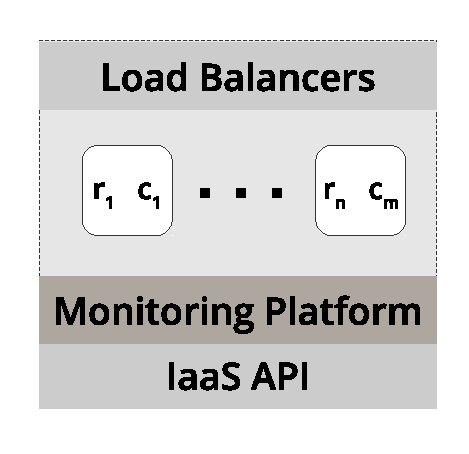
\includegraphics[scale=0.7]{figs/deployment}
%\end{center}
%\vspace{-20pt}
%\caption{{\footnotesize High-level deployment architecture}}
%\label{fig:deployment}
%\vspace{-10pt}
%\end{wrapfigure}
%Figure \ref{fig:deployment} presents a high-level overview of services deployed in a distributed environment (e.g. ``the cloud'').
In the deployment environment (e.g., ``the cloud''), every  server from the IaaS provider is  used for a \emph{single} service of a customer, such as
the Query Service API for a customer of SDL Fredhopper (c.f. Section \ref{sec:fredhopper_example}).
Typically, multiple servers are allocated to a single customer.
The number of servers allocated for a customer is not visible to the customer.
The customer uses a single endpoint - in the load balancer layer - to access all their services.

The ultimate goal is to maintain the environment in such a way that customers and their end users experience the delivered services up to their expectations while minimizing the cost of the system.
%environment does not have a negative impact on the business of SDL Fredhopper.
The first objective can be addressed by adding resources; however, this conflicts with the second goal since it increases the cost of the environment for the customer.
In this section, we formalize the above intuitive notions as \emph{service availability} and \emph{service budget compliance}.

We then develop a distributed monitoring platform that aims to optimize these service
characteristics in a deployment environment.
 % given in Figure \ref{fig:deployment}.
The monitoring platform works in two cyclic phases: \emph{observation} and \emph{reaction}.
The observation phase takes measurements on services in the deployment environment.
Subsequently, the corresponding levels of the service characteristics are calculated.
In the reaction phase, if needed, a platform API is utilized to make the necessary changes to the deployment environment (e.g. adjust the number of allocated resources) to optimize the service characteristics.
% In the monitoring platform, not all components reside in the same resource in the deployment environment; all communications and interactions are performed in an \emph{asynchronous} way.
The monitoring platform builds on top of a real-time extension of the 
actor-based language ABS~\cite{johnsen2012abs}.
To ensure non-intrusiveness of the monitor with the running service,
each monitor is an active object (actor) running on a separate resource
from that which runs the service itself, and the components of the monitoring platform communicate through \emph{asynchronous messages} with deadlines~\cite{johnsen2012modeling}.
% The following elements are the major high-level components of the monitoring platform:
%for a distributed deployment environment: 

Below, we discuss assumptions and basic oncepts that will be used in the
analysis of the formal properties of the monitoring platform and corresponding theorems.
We assume that the external infrastructure provider has an  \emph{unlimited} number of resources.
Further, we assume that all resources are of the \emph{same type}; i.e. they have the same computing power, memory, and IO capacity.
Finally, we assume that every resource   is initialized within  at most $t_i$ amount of time.
%We illustrate and motivate each assumption and definition and discuss how they are generalized from real use-cases from the large deployment environment of the
%SDL Fredhopper cloud.

%\begin{assm}[Unlimited Capacity]
%\label{def:platform:cap}
%We assume that the external infrastructure provider is capable to provision an \emph{unlimited} number of resources.
%\end{assm}

%In reality, every service provider such as SDL Fredhopper has a separate contract with an IaaS provider such as AWS.
%In these contracts, there cannot be a guarantee for \emph{unlimited} capacity.
%We simplify this limitation by assuming that the platform API (IaaS layer abstraction) is capable to provision as many resources as requested.

%\begin{assm}[Single Resource Type]
%\label{def:single:resource:type}
%To simplify reasoning, we assume that all resources are of the \emph{same type}; i.e. they have the same computing power, memory, and IO capacity.
%For example, if we are using AWS,
%we could choose the instance type \jtt{m1.large} for all the services.
%\end{assm}

%If a business delivers different types of services, it cannot avoid the fact that different services may require different \emph{capabilities} from their underlying resources.
%% i.e. one service might require high I/O throughput for its process whereas another might demand high parallelism support from the hardware.
%% Such capability profiles are provisioned through different types of resources from a IaaS provider.
%For example, AWS offers\footnote{\url{http://aws.amazon.com/ec2/instance-types/}} families of EC2 instance types each of which expose different sets of capabilities in terms of computation power, I/O, and network.
%We simplify our analysis by assuming that there is a \emph{single resource type} that is able to provide the necessary capabilities for all services.% in this research scope.

%\begin{assm}[Resource Initialization Time $t_i$]
%\label{def:resource:init:time}
%We assume that every resource $r$ that is initialized is ready for use in at most $t_i$ amount of time.
%% The time $t_i$ is bounded by a finite constant value.
%\end{assm}

%Initialization time can vary between different resource types. The above Assumption \ref{def:single:resource:type} simplifies this: we can just choose the initialization time (a fixed constant) of the single resource type that was chosen.
%The initialization time is also part of the contract with the IaaS provider.
%As discussed above in Assumption \ref{def:single:resource:type}, when a resource is launched and initialized, it might take a different amount of time to be in a state that is \emph{operational} and ready to be used.
%Thus,
%We simplify the property of initialization time of a resource to be a fixed constant for the single resource type that is used in the context of this research.

In our framework
time $T$ is a universally shared clock based on the NTP
\footnote{\url{https://tools.ietf.org/html/rfc1305}} that is used by all elements of the system in the same way. 
$T$ is discrete.
We fix that the unit of time is \emph{milliseconds}.
This level of granularity of time unit means that between
two consecutive milliseconds, the system is not observable.
For example, we use the UTC time standard for all services, monitors and platform API.
We refer to the current time by $t_c$.

We denote by $r$ a resource which provides computational power and storage
and by $s$ a general abstraction of a service in the deployment environment. 
A service exposes an API that is accessible through a delivery layer, such as HTTP.
In our example, a service is the Query API (c.f. Section~\ref{sec:fredhopper_example}) that is accessible through a single HTTP endpoint.

In our framework, 
\emph{monitoring platform}  $P$ is responsible for (de-)allocation of resources for computation or storage.
We abstract from a specific implementation of the monitoring platform $P$ through an API in Listing~\ref{lst:platform}. 
% 
\lstset{language=java,aboveskip=-20pt,belowskip=-20pt}
\begin{wrapfigure}{r}{0.5\textwidth}
\vspace{-15pt}
\begin{center}
\begin{lstlisting}[mathescape,caption=Platform API,label=lst:platform]
interface Platform {
  void    allocate(Service s);
  void    deallocate(Service s);
  Number  getState(Service s);
  boolean verify$_\alpha$(Service s);
  boolean verify$_\beta$(Service s);
}
\end{lstlisting}
\end{center}   
\vspace{-15pt}
\end{wrapfigure}
% 
There is only \emph{one} instance of $P$ available.
In this paper, $P$ internally uses an external infrastructure provisioning API to provide resources (e.g. AWS EC2).
The term ``platform'' is interchangeably used for monitoring in this paper.
The platform provides a method \jtt{getState(Service s)} which returns
the number of resources allocated to the given service $s$ at time $t_c$.

%Monitoring is a runtime analysis approach~\cite{Logean_monitoring}.
We use monitoring to observe the external behavior of a service.
We formalize the external behavior of a service with its service-level agreement (SLA).
An SLA is a contract between the customer (service consumer) and the service provider
which defines (among other things) the minimal quality of the offered service,
and the compensation if this minimal level is not reached.
To formally analyze an SLA, we introduce the notion of a service metric function.
We make basic measurements of the service externally in a given monitoring window (a duration).
The service metric function aggregates the basic measurements into a single number
that indicates the quality of a certain service characteristic (higher numbers are better).
%
%monitoring window measurement.
%The quantified measurements projected to a monitoring window lead to an understanding of the quality of the service based on its SLA.

\emph{Basic measurement} $\mu(s,r,t)$ is a function that produces a real number of a \emph{single} monitoring check on a resource $r$ allocated to service $s$ at some time $t$.  
For example, for SDL Fredhopper cloud services, a basic measurement is the number of completed queries at the current time. 
% 

\emph{Service Metric} $f_s$ is a function that aggregates a sequence of basic non-negative measurements to a single non-negative real value:
$f_s : \bigcup_n \mathbb{R}^n \rightarrow \mathbb{R}$.
For example, for SDL Fredhopper cloud services, the service metric function
$f_s$ calculates the average number of queries per second (\qps) given a list of basic measurements.

\emph{Monitoring Window} is a duration of time $\tau$ throughout which basic measurements for a service are taken.
% 

\emph{Monitoring Measurement} is a function that aggregates the basic measurements for a service over its resources in the last monitoring window.
The last monitoring window is defined as $[t_c-\tau, t_c]$.
To produce the monitoring measurement, $f_s$ is applied.
Formally:
\[
\mu(s,r,\tau) = 
f_s \big(\langle \mu_i(s,r,t) \rangle^{\infty}_{i=0}\big) \;\; \textnormal{where} \;\; t \in [t_c-\tau, t_c] 
\]
in which $\mu_i(s,r,t)$ is the $i$-th basic measurement of services $s$ on resource $r$ at time $t$ where $t \in [t_c-\tau,t_c]$.


\begin{defn}[Service Availability $\alpha(s,\tau,t_c)$]
\label{def:service:availability}
% 
First, we need a few auxiliary definitions before we can define service availability.
% 


\emph{Service Capacity} $\kappa_\sigma(s,\tau) = \sum_{r \in \sigma(s)} \mu(s,r,\tau)$ denotes the  capability of service $s$ that is the aggregated monitoring measurements of its resources over the monitoring window $\tau$ and $\sigma(s)$ is the number of allocated resources to service $s$.
% 

\emph{Agreement Expectation} $E(s,\tau, t_c)$ is the minimum number of requests that a customer expects to complete in a monitoring window $\tau$.
The agreement expectation depends on the current time $t_c$ because the expectation may change over time.
For example, SDL Fredhopper customers expect a different \qps during Christmas.
% 

We define the availability of a service $\alpha(s,\tau,t_c)$ in every monitoring window $\tau$ as:
\vspace{-10pt}
\[
\alpha(s,\tau,t_c) = \frac{\kappa_\sigma(s,\tau)}{E(s,\tau,t_c)}
\]
% in every monitoring window $\tau$.
% 

\emph{Capacity Tolerance} $\varepsilon_\alpha(s,\tau)) \in [0,1]$ defines how much $\kappa_\sigma(s,\tau)$ can deviate from $E(s,\tau,t_c)$ in every time span
of duration $\tau$.
\end{defn}
% 

\emph{Service Guarantee Time $t_G$} is the duration within which a customer expects service availability reaches an acceptable value after a violation. 
Typically, $t_G$ is an input parameter from the customer's contract.


\begin{exmp}
Intuitively, $\alpha(s,\tau,t_c)$ presents the actual capability of a service $s$ over a time period $\tau$ compared to the expectation on the service $E(s,\tau)$. 
For values $\alpha(s,\tau,t_c) \ll 1 - \varepsilon_\alpha(s,\tau))$, the resource for service $s$ are at ``under-capacity'' while for values $\alpha(s,\tau,t_c) \gg 1 + \varepsilon_\alpha(s,\tau))$, there is ``over-capacity''. The goal is optimize $\alpha(s,\tau,t_c)$ towards a value of 1.
% 

For example, we expect a query service to be able to complete 10 queries per second. 
We define the monitoring window $\tau = $ 5 minutes; thus, $E(s,\tau,t_c) = 10 \times 60 \times 5 = 3000$.
Suppose we allocate only one resource to the service,
measure the service during a single monitoring window $\tau$
and find $\mu(s,r,\tau) = 2900$. Then $\alpha(s,\tau,t_c) = \frac{2900}{3000} = 0.966$.
If we have $\varepsilon_\alpha(s,\tau)) = 0.03$, this means that service $s$ is under-capacity because $\alpha(s,\tau,t_c) < 1 - \varepsilon_\alpha$.
\end{exmp}

\begin{defn}[Budget Compliance $\beta(s,\tau)$]
\label{def:budget:compliance}
% 
We first provide a few auxiliary definitions.
% 

\emph{Resource Cost} $\euro(r,\tau) \in \mathbb{R}^+$ is the cost of resource $r$ in a monitoring window $\tau$ which is determined by a fixed resource cost per time unit.

\emph{Service Cost} $\euro_\sigma(s,\tau) \in \mathbb{R}^+$ is the cost of a service $s$ in a monitoring window $\tau$ and defined as $\euro_\sigma(s,\tau) = \sum_{r \in \sigma(s)} \euro(r,\tau)$.
% 

\emph{Service Budget} $B(s,\tau)$ specifies an upper bound of the expected cost of a service in the time span $\tau$.
Intuitively $B(s,\tau)$ is the allowed budget that can be spent for service $s$ over the time span $\tau$.
%Note that
The service budget is typically chosen to be fixed over any time span $\tau$.
% 

We are now ready to define service budget compliance $\beta(s,\tau)$ that,
intuitively, represents how a service complies with its allocated budget:
\[
\beta(s,\tau) = \frac{\euro_\sigma(s,\tau)}{B(s,\tau)}
\]

\emph{Budget Tolerance} $\varepsilon_\beta(s,\tau) \in [0,1]$ specifies how much the service cost $\euro(s,\tau)$ can deviate from $B(s,\tau)$ in every time span of duration $\tau$.

\emph{Service Guarantee Time} $t_G$ is similar to that defined for service availability.
% 
\end{defn} % end - budget compliance

\begin{exmp}
% during its runtime. 
Assume every resource on the environment costs $1$ (e.g. $\euro$) per hour.
Suppose we set a budget of $1.5$ per hour for every service,
allocate \emph{one} resource to the service and define a monitoring window of $\tau = 5$ minutes.
Every hour has $12$ monitoring windows.
This means that each resource costs $\euro(r,\tau) = \frac{1}{12} \approx 0.08$ per monitoring window.
Since there is only one resource, the service cost is $\euro(s,\tau) = \sum_{r\in\sigma(s)}\euro(s,\tau) \approx 0.08$ per monitoring window.
On the other hand, if we calculate the budget for one monitoring window, we have $B(s,\tau) = \frac{1.5}{12} = 0.125$ per monitoring window.
This yields budget compliance as $\beta(s,\tau) = \frac{0.08}{0.125} = 0.64$.
\end{exmp}
% 

% The formal definitions above provide a basis
% to react appropriately to changes or failures in an environment.
% We enumerate a few as follows.
% 
% A service $s$ is ``under-capacity'' as long as $\alpha(s,\tau,t_c) < 1 - \varepsilon_\alpha(s,\tau))$; 
% i.e. intuitively this means that the service cannot provide the expected quality to
% end-users.
% To fix an under-capacity service, \emph{new} resources through the monitoring platform $P$ can be requested (scale up) to increase the capacity of $s$.
% Similarly, service $s$ can be ``over-capacity'';
% i.e. $\alpha(s,\tau,t_c) \gg 1 + \varepsilon_\alpha(s,\tau))$.
% An important disadvantage of an over-capacity service is that it \emph{costs} more than necessary to deliver what is expected from it.
% To improve an over-capacity service, at least one of the current resources allocated to service $s$ can be terminated (scale down) as long as this does not result in an ``under-capacity'' service.
%Similarly, a service can be ``over-budget'' and ``under-budget'', and corresponding actions can be taken to resolve that.

The formal definitions of service availability and budget compliance provide a rigorous 
basis for automatic deployment of resource-aware services with an appropriate quality of service, taking costs into account.
%Properties $\alpha(s,\tau,t_c)$ and $\beta(s,\tau)$ of a service $s$ build a foundation facilitate \emph{automation of operation} of the service according to its properties. 
This in particular includes automated scaling up or down of the service with the help of monitoring checks that are installed for the service. 
%However,
The fundamental challenge in ensuring service availability and budget compliance is that they have \emph{conflicting} objectives:
\[
\alpha(s,\tau,t_c) \uparrow \iff \beta(s,\tau) \downarrow
\]
Intuitively, if more resources are used to ensure the availability of a service; then $\alpha(s,\tau,t_c)$ increases.
However, at the same time, the service costs more; i.e. budget compliance $\beta(s,\tau)$ decreases.

% In the following sections, we first present two separate timed automata~\cite{alur:1994:timedautomata} to model the behavior of $\alpha(s,\tau,t_c)$ and $\beta(s,\tau)$.
% Then, we formalize how the two can be composed to form a new property called service sustainability $\gamma(s,\tau)$.

% In the next section, we design a timed automata for each service characteristics.
% We show how the timed automata can be used to evolve the systems towards SLA optimizations.
% We present a generalization of the characteristics and how they can be composed together.

% -*- root: paper-esocc.tex -*-

\section{Service Characteristics Verification}
\label{ch04:sec:timed:fsm}

In this section, we use timed automata and task automata to model the behavior of a monitoring platform $P$, the deployment environment $E$, and the monitoring components for service availability $\alpha(s,\tau,t_c)$ and budget compliance $\beta(s,\tau)$. 
\cite{jaghoori2010time} defines a task automata as an extension of timed automata in which each task is a piece of executable program with $(b,w,d)$: best/worst time and deadline of the task. A task automata uses a scheduler for the tasks to schedule each task with a location on a queue.
% 

Modeling the elements of the monitoring platform is necessary to be able to study certain properties of the system.
The most important goal of a monitoring platform is to enable the autonomous operation of a set of services according to their SLA.
Thus, it is essential how to analyze that the monitoring platform can provide certain guarantees about the service and its SLA.
In addition, it is important be able to verify the monitoring platform through model checking and schedulability analysis.
Using timed automata and task automata facilitates model checking and verification through formal method tools such as UPPAAL~\cite{uppaal2004} supporting advanced methods such as state-space reduction~\cite{larsen1997efficient}. 
   
We use task automata as defined in \cite{fersman2007task,jaghoori2012composing,jaghoori2010time}.
Task automata are an extension of timed automata~\cite{alur:1994:timedautomata}.
In addition, we design the automata for the monitoring platform using the real-time extension of task automata presented in \cite{jaghoori2010time} p. 92 in which the author presents a mapping from Real-Time ABS~\cite{johnsen2012modeling} to the equivalent task automata.

A task type is a piece of executable program/code represented by a tuple $(b,w,d)$, where $b$ and $w$ respectively are the best-case and worst-case execution times and $d$ is the deadline.
In a task automata, there are two types of transitions: \emph{delay} and \emph{discrete}.
A delay transition models the execution of a running task by idling for other tasks.
A discrete transition corresponds to the arrival of a new task.
When a new task is triggered, it is placed into a certain position in the queue based on a scheduling policy~\cite{Nobakht:sched,nobakht2013future}.
Examples of a scheduling policy are \textsf{FIFO} or \textsf{EDF} (earliest deadline first).
The scheduling policy is modeled as a timed automaton \textsf{Sch}.
Every task has its own stop watch.
The scheduler also maintains a separate stop watch for each task to determine if a task misses its deadline.
All stop watches work at the same clock speed specified by $T$.

We design separate automata for each service $s$ characteristic: service availability $\alpha(s,\tau,t_c)$ by an automata $M_{\alpha_s}$ and service budget compliance $\beta(s,\tau)$, by an automata $M_{\beta_s}$.
Each automaton is responsible for one goal: to optimize the service characteristic.
$M_{\alpha_s}$ aims to improve $\alpha(s,\tau,t_c)$ whereas $M_{\beta_s}$ aims to improve $\beta(s,\tau)$.
$M_{\alpha_s}$ uses \jtt{allocate} to launch a new resource in the environment and improve the service $s$.
In contrast, $M_{\beta_s}$ uses \jtt{deallocate} to terminate a resource to decrease the cost of the service.

We use task automata to design $M_{\alpha_s}$.
Periodically, $M_{\alpha_s}$ checks whether the service availability
is within the thresholds, taking tolerance into account
(Definition~\ref{ch04:def:service:availability}).
If the condition fails, $M_{\alpha_s}$ generates a task for monitoring platform $P$ to allocate a new resource to service $s$ with a deadline of $\tau$.
We define the period to be $\tau$.
We use the semantics of a task automata in \cite{jaghoori2010time} p. 92 in the transitions of the task automata.
Figure~\ref{ch04:fig:fsm:task:alpha} and \ref{ch04:fig:fsm:task:beta} present $M_{\alpha_s}$ and $M_{\beta_s}$.
Both $M_{\alpha_s}$ and $M_{\beta_s}$ share state with the monitoring platform $P$.
The state keeps the current number of resources for a service $s$ that is denoted by $\sigma(s)$.
All timed automata and task automata in the monitoring platform have shared access to $\sigma(s)$.
In the automata, we use a conditional statement to check the service characteristics $\alpha(s,\tau,t_c)$ or $\beta(s,\tau)$.
If the condition fails, $M_{\alpha_s}$ requests $P$ to \jtt{allocate} a new resource to $s$ and $M_{\beta_s}$ requests $P$ to \jtt{deallocate} a resource.
In addition, $M_{\alpha_s}$ triggers a new task $\jtt{verify}_\alpha$ with deadline $t_G$.
Intuitively, this means the service characteristic $\alpha(s,\tau,t_c)$ is verified to be within the expected thresholds after at most $t_G$ time.

\begin{figure}[h]
% \vspace{-15pt}
\captionsetup[subfigure]{font=footnotesize}
\centering
\subcaptionbox{\scriptsize{$M_{\alpha_s}$ task automata for $\alpha(s,\tau,t_c)$}\label{ch04:fig:fsm:task:alpha}}[0.45\textwidth]{
\begin{tikzpicture}[->,>=stealth',shorten >=1pt,auto,node distance=7cm,thick,scale=0.6,every node/.style={scale=0.6},level distance=20mm]
\node[state,initial]
  (a)   {};
\node[state]
  (b) [right of=a]  {};
\path[]
(a)
  edge
  node {$\bfjtt{duration}(\tau,\tau)$}
  (b)
(b)
  edge [bend right,above] 
  node [align=center] 
    {$\bfjtt{if}\big((1-\varepsilon_\alpha(s,\tau,t_c)) > \alpha(s,\tau,t_c)\big) $ \\ \{ %\\
     $P \; ! \; \jtt{allocate}(s,\tau)$ ; %\\
     $P \; ! \; \jtt{verify}_\alpha(s,t_G)$ \}
    }
  (a)
;
\end{tikzpicture}
}%
\subcaptionbox{\scriptsize{$M_{\beta_s}$ task automata for $\beta(s,\tau)$}\label{ch04:fig:fsm:task:beta}}[0.45\textwidth]{
\begin{tikzpicture}[->,>=stealth',shorten >=1pt,auto,node distance=7cm,thick,scale=0.6,every node/.style={scale=0.6},level distance=20mm]
\node[state,initial]
  (a)   {};
\node[state]
  (b) [right of=a]  {};
\path[]
(a)
  edge 
  node {$\bfjtt{duration}(\tau,\tau)$}
  (b)
(b)
  edge [bend right, above] 
  node [align=center] 
       {$\bfjtt{if}\big((1-\varepsilon_\beta(s,\tau)) > \beta(s,\tau)\big) $ 
       \\ \{ %\\
        $P \; ! \; \jtt{deallocate}(s,\tau)$ ; %\\
        $P \; ! \; \jtt{verify}_\beta(s,t_G)$ \}
       }
  (a)
;
\end{tikzpicture}
}
% \vspace{-10pt}
% \vspace{-10pt}
\caption{{\scriptsize Task Automata for $\alpha(s,\tau,t_c)$ and $\beta(s,\tau)$}}
\end{figure}

We use a separate task automaton for each service characteristic to verify the SLA of the service after $t_G$ time.
Respectively, $M^{\alpha}_{\jtt{V}}$ and $M^{\beta}_{\jtt{V}}$ execute tasks $\jtt{verify}_\alpha$ and $\jtt{verify}_\beta$ (Figures~\ref{ch04:fig:fsm:task:verify:alpha} and \ref{ch04:fig:fsm:task:verify:beta}).
$M^{\alpha}_{\jtt{V}}$ uses \bfjtt{await} to ensure the condition of the SLA.
In addition, the task is controlled by the scheduler using a deadline that is specified as $t_G$ in the generated task $\jtt{verify}_\alpha(s,t_G)$ in $M_{\alpha_s}$. 
If $t_G$ passes before the guard statement in \bfjtt{await} statement holds, it leads to a \emph{missed deadline}.

\begin{figure}[h]
% \vspace{-20pt}
\captionsetup[subfigure]{font=scriptsize}
\centering
\subcaptionbox{\scriptsize{$M^{\alpha}_{\jtt{V}}$ to execute $\jtt{verify}_\alpha$}\label{ch04:fig:fsm:task:verify:alpha}}[0.45\textwidth]{
\begin{tikzpicture}[->,>=stealth',shorten >=1pt,auto,node distance=6.5cm,thick,scale=0.6,every node/.style={scale=0.6},level distance=20mm]
\node[state,initial]
  (a)   {};
\node[state,accepting]
  (b) [right of=a]  {};
\path[]
(a)
  edge
  node [align=center] 
    {$\bfjtt{await} \; \alpha(s,\tau,t_c) \geq 1-\varepsilon_\alpha(s,\tau,t_c)$}
  (b)
;
\end{tikzpicture}
}%
\subcaptionbox{\scriptsize{$M^{\beta}_{\jtt{V}}$ to execute $\jtt{verify}_\beta$}\label{ch04:fig:fsm:task:verify:beta}}[0.45\textwidth]{
\begin{tikzpicture}[->,>=stealth',shorten >=1pt,auto,node distance=6cm,thick,scale=0.6,every node/.style={scale=0.6},level distance=20mm]
\node[state,initial]
  (a)   {};
\node[state,accepting]
  (b) [right of=a]  {};
\path[]
(a)
  edge
  node [align=center] 
    {$\bfjtt{await} \; \beta(s,\tau) \geq 1-\varepsilon_\beta(s,\tau)$}
  (b)
;
\end{tikzpicture}%
}
% \vspace{-10pt}
% \vspace{-10pt}
\caption{{\scriptsize Task automata to execute $\jtt{verify}_\alpha$ and $\jtt{verify}_\beta$}}
\end{figure}

Both $M_{\alpha_s}$ and $M_{\beta_s}$ are specific to one particular service $s$.
A generalized automaton for all services is obtained as their parallel composition:$M_\alpha = (\parallel_s M_{\alpha_s})$ and $M_\beta = (\parallel_s M_{\beta_s})$.
The tasks generated by $M_\alpha$ and $M_\beta$ (triggered by the calls to
\jtt{allocate} and \jtt{deallocate}) are executed by the task automata for platform $M_P$.

We model monitoring platform $P$ by a task automata $M_P$.
The task types are $\{\jtt{A}(\jtt{allocate}),\allowbreak \jtt{D}(\jtt{deallocate})\}$.
For task type \jtt{A} in $M_P$, we use $(b,w,d) = (t_i,\tau,\tau)$; i.e.
the best-case execution time of a task is the resource initialization time, 
the worst-case is the length of the monitoring window, and
the deadline is the length of the monitoring window.
For task type \jtt{D} in $M_P$, we use $(b,w,d) =(0, \tau,\tau)$. 
We do not fix the scheduling policy \textsf{Sch}.
The error state $q_{err}$ in $M_P$ is defined when either a deadline is missed or when the platform fails to provision a resource.
Thus the monitoring platform $P$ contains the following ingredients:
\[
M_P = \langle M_{\jtt{A}} \parallel M_{\jtt{D}} \parallel 
M^{\alpha}_{\jtt{V}} \parallel M^{\beta}_{\jtt{V}}
, \textsf{Sch}, \tau \rangle
\]
We define $M_{\jtt{A}_s}$ as the timed automata to execute the tasks of type \jtt{allocate} in $M_P$.
We use the model  semantics presented in \cite{jaghoori2010time} p. 92 to design $M_{\jtt{A}_s}$. The resulting automata is presented in Figure~\ref{ch04:fig:fsm:alloc_s}.

\begin{figure}[h]
% \vspace{-20pt}
\centering
\begin{tikzpicture}[->,>=stealth',shorten >=1pt,auto,node distance=4cm,thick,scale=0.7,every node/.style={scale=0.7}]
\node[state,initial]    
  (a)   {};
\node[state]
  (b) [right of=a]   {};
\node[state,accepting]
  (c) [right of=b]  {};
\path[]
(a) 
    edge    
    node {$\bfjtt{duration}(t_i,\tau)$}          
    (b)
(b) 
    edge    
    node {$\sigma(s) \gets \sigma(s) + 1$} 
    (c)
;
\end{tikzpicture}
% \vspace{-15pt}
\caption{$M_{\jtt{A}_s}$: Timed Automaton to execute task type \jtt{allocate} in $M_P$}
% \vspace{-20pt}
\label{ch04:fig:fsm:alloc_s}
\end{figure}

Then, we define $M_{\jtt{A}}$ in $M_P$ as:
$M_{\jtt{A}} = \; \parallel_s M_{\jtt{A}_s}$; i.e.
the composition of all timed automata to execute a task \jtt{allocate} for some service $s$.
% 
Similarly, we design $M_{\jtt{D}_s}$ to execute task type \jtt{deallocate} in Figure~\ref{ch04:fig:fsm:dealloc_s}.
Therefore, we also have $M_{\jtt{D}}$ in $M_P$ as: $M_{\jtt{D}} = \; \parallel_s M_{\jtt{D}_s}$.
% 
\begin{figure}[h!]
% \vspace{-10pt}
\centering
\begin{tikzpicture}[->,>=stealth',shorten >=1pt,auto,node distance=4cm,thick,scale=0.7,every node/.style={scale=0.7}]
\node[state,initial]    
  (a)   {};
\node[state]
  (b) [right of=a]   {};
\node[state,accepting]
  (c) [right of=b]  {};
\path[]
(a) 
    edge    
    node {$\bfjtt{duration}(t_i,\tau)$}          
    (b)
(b) 
    edge    
    node {$\sigma(s) \gets \sigma(s) - 1$} 
    (c)
;
\end{tikzpicture}
% \vspace{-15pt}
\caption{$M_{\jtt{D}_s}$: Timed Automaton to execute task type \jtt{deallocate} in $M_P$}
% \vspace{-20pt}
\label{ch04:fig:fsm:dealloc_s}
\end{figure}
% 

For a particular service $s$, its automaton $M_{\alpha_s}$ regularly measures the service
characteristics and calculates $\alpha(s,\tau,t_c)$. When $s$ is under-capacity, $M_{\alpha_s}$ requests to \jtt{allocate} a new resource for $s$ through monitoring platform $P$.
This generates a new task in $M_P$ that is executed by $M_{\jtt{A}_s}$.
When the task completes, the state of the service $\sigma(s)$ is updated; strictly increased.
Thus, in isolation, the combination of $M_{\alpha_s}$ and $M_{\jtt{A}_s}$ increase the value of service availability $\alpha(s,\tau,t_c)$ for service $s$ over time.
Similarly, in isolation, the combination of $M_{\beta_s}$ and $M_{\jtt{D}_s}$ increase the value of service budget compliance $\beta(s,\tau)$ for service $s$ over time. 
Because in the latter, \jtt{deallocate} is used to decrease the cost of the service and as such increases $\beta(s,\tau)$. 

In reality, resources might fail in the environment.
The failure of a resource is not and cannot be controlled by the monitoring platform $P$.
However, the failure of a resource affects the state of a service and its characteristics.
Thus, we model the environment, including failures, as an additional timed automata, $M_E$.
In $M_E$, in every monitoring window, there is a probability that some resources fail.
For example, we present a particular instance of $M_E$ in Figure~\ref{ch04:fsm:env}.
In this environment, in every monitoring, an unspecified constant ($c$) number of resources fail.

\begin{figure}[h]
% \vspace{-20pt}
\centering
\begin{tikzpicture}[->,>=stealth',shorten >=1pt,auto,node distance=5cm,thick,scale=0.7,every node/.style={scale=0.7}]
\node[state,initial]
  (a) {};
\node[state]
  (b) [right of=a] {};
\node[state]
  (c) [right of=b] {};
\path[]
(a)
  edge
  node {$\bfjtt{duration}(0,\tau)$}
  (b)
(b)
  edge
  node {$\sigma(s)\gets\sigma(s)-c$}
  (c)
;
\end{tikzpicture}
% \vspace{-13pt}
\caption{An example behavior for $M_E$}
\label{ch04:fsm:env}
% \vspace{-20pt}
\end{figure}

We define system automata~\cite{jaghoori2010time} (p. 33, Definition 3.2.7) for each service characteristic;
$\mathcal{S}_\alpha$ for $\alpha(s,\tau,t_c)$ and $\mathcal{S}_\beta$ for $\beta(s,\tau)$:
\[
\mathcal{S}_\alpha = M_\alpha \parallel M_E \parallel M_P
\quad\quad\textit{ and }\quad\quad
\mathcal{S}_\beta = M_\beta \parallel M_E \parallel M_P
\]

With the above automata that we designed for $\alpha(s,\tau,t_c)$ and $\beta(s,\tau)$, we are now ready to present the main results.
% 

\begin{thm}
\label{ch04:thm:alpha}
If the SLA for service $s$ on $\alpha(s,\tau,t_c)$ is violated, either:
\begin{itemize}
\item $\mathcal{S}_\alpha$ re-establishes the condition $\alpha(s,\tau,t_c) \geq 1 - \varepsilon_\alpha(s,\tau)$ (thereby satisfying the SLA) within $t_G$ time, or, 
\item there exists at least one task $\jtt{verify}_\alpha$ in $M^{\alpha}_{\jtt{V}}$ with a missed deadline.
\end{itemize}
\end{thm}

\begin{proof}
At any given time in $T$:
\begin{itemize}
\item If $\alpha(s,\tau,t_c) \geq 1-\varepsilon_\alpha(s,\tau)$, then the SLA for service availability $\alpha$ is satisfied. 
\item If the above condition does not hold, on every monitoring window $\tau$, $M_\alpha$ generates a new task \jtt{allocate} in $M_{\jtt{A}}$. 
In addition, a new task $\jtt{verify}_{\alpha}$ is generated with a deadline $t_G$. 
After a duration of $t_G$, the \bfjtt{await} statement allows $M^{\alpha}_{\jtt{V}}$ to complete the task $\jtt{verify}_\alpha$ only if the condition $\alpha(s,\tau,t_c) \geq 1-\varepsilon_\alpha(s,\tau)$ holds.
If this is not the case, since $t_G$ has passed, the scheduler generates a missed deadline (moving to its error state). 
\end{itemize}
\end{proof}

\begin{thm}
\label{ch04:thm:beta}
If the SLA for service $s$ on $\beta(s,\tau)$ is violated, either:
\begin{itemize}
\item $\mathcal{S}_\beta$ re-establishes the condition $\beta(s,\tau) \geq 1-\varepsilon_\beta(s,\tau)$ (thereby satisfying the SLA) within $t_G$ time, or,
\item there exists at least one task $\jtt{verify}_\beta$ in $M^{\beta}_{\jtt{V}}$ with a missed deadline. 
\end{itemize}
\end{thm}

\begin{proof}
Similar to the proof of Theorem~\ref{ch04:thm:alpha}.
\end{proof}

In practice, the guarantee of $\mathcal{S}_\alpha$ and $\mathcal{S}_\beta$
in isolation to eventually evolve the system to satisfy the SLA is not enough.
In reality, a service provider tries ensure both simultaneously to reduce their cost of service delivery while ensuring the delivered service is of the expectations agreed upon with the customer.
However, these goals conflict.
When $\alpha(s,\tau,t_c)$ increases because of adding a new resource,
it means that service $s$ costs more, hence $\beta(s,\tau)$ decreases.
%Under the same $B(s,\tau)$, this means that $\beta(s,\tau)$ decreases.
The same applies in the other direction: increasing $\beta(s,\tau)$
negatively affects $\alpha(s,\tau,t_c)$.

To capture the combined behavior of service availability and budget compliance,
we compose them. 
We define \emph{service sustainability} $\gamma(s,\tau)$ as the composition of $\alpha(s,\tau,t_c)$ and $\beta(s,\tau)$.
We present the composition by system automata $\mathcal{S}_\gamma$ as:
\[
\mathcal{S}_\gamma = \mathcal{S}_\alpha \; \parallel \; \mathcal{S}_\beta
\]

Authors in~\cite{fersman2007task} define that a task automata is \emph{schedulable} if there exists no task on the queue that misses its deadline. 
The next theorem presents the relationship between schedulability analysis of service sustainability and satisfying its SLA.

\begin{thm}
\label{ch04:thm:gamma}
If $\mathcal{S}_\gamma$ is \emph{schedulable} given input parameters $(\tau, t_i, t_G)$, then the SLA for both service characteristics $\alpha(s,\tau,t_c)$ and $\beta(s,\tau)$ is satisfied within $t_G$ time after a violation.
\end{thm}

\begin{proof}
When a violation of the SLA occurs in $\mathcal{S}_\gamma$, either $\mathcal{S}_\alpha$ or $\mathcal{S}_\beta$ (or both) start to evolve the service based on Theorems~\ref{ch04:thm:alpha} and \ref{ch04:thm:beta}.
Therefore, there exists at least one task of $\jtt{verify}_\alpha$ or $\jtt{verify}_\beta$ with a deadline $t_G$.
% 
Hence, if $\mathcal{S}_\gamma$ is schedulable, then neither $\jtt{verify}_\alpha$ nor $\jtt{verify}_\beta$ miss their deadline.
Thus, both $\mathcal{S}_\alpha$ and $\mathcal{S}_\beta$ are schedulable.
This means that both $\jtt{verify}_\alpha$ and $\jtt{verify}_\beta$ complete successfully.
Therefore, the SLA of the service is guaranteed within $t_G$ after a violation in $\mathcal{S}_\gamma$.
\end{proof}

Using the algorithm presented in Chapter 6~\cite{jaghoori2010time}, we translate the above task automata into traditional timed automata.
This allows to leverage well-established model checking techniques such as UPPAAL~\cite{uppaal2004} to determine the schedulability of $\mathcal{S}_\gamma$.
Moreover, the results of the schedulability analysis serves as a method to optimize the input parameters of the monitoring model including $\tau$ and $t_G$.
% -*- root: paper-esocc.tex -*-

\section{Evaluation of the monitoring model} % (fold)
\label{sec:implementation}

In this section, we evaluate the implementation of the monitoring model.
% that we presented in the previous sections.

We set up an environment to evaluate how the monitoring evolves a service according to its SLA. 
In the environment, a single instance of monitoring platform is present to provide new resources as necessary.
Every resource hosts only one service.
We define two customers in the environment.
For both customers, we deploy the same service, Fredhopper Query API.
For every resource that hosts a service, we set up a monitor that measures \qps and reports it to the platform.
Both customers run with the same SLA: the \qps expectation is $E(s,\tau,t_c) = 10$ and $\varepsilon_\alpha(s,\tau,t_c) = 0.1$.
We launch every customer service with only one resource.
Monitors observe the customer service and calculate the service availability of every customer service $\alpha(s,\tau,t_c)$.

We run the environment setup for different monitoring windows $\tau \in \{1,5,10\}$ (seconds).
We fix the initialization time of a resource to $t_i = 2.5$ seconds.
We set $t_G = 300$ seconds; i.e. we verify the service after this time and evaluate if the service is guaranteed based on its SLA. 

Figure~\ref{fig:alpha} plots the service availability $\alpha(s,\tau,t_c)$ over time with the different monitoring windows.
The following summarizes the behavior:
\begin{itemize}
\item As the monitoring window $\tau$ increases, the system converges with a slower pace towards the expected $\alpha(s,\tau,t_c)$.
\item When the monitoring window is chosen such that $\tau < t_i$, the evolution of the system becomes \emph{non-deterministic}.
\item The setting $\tau < t_i$ causes a missed deadline in $\jtt{verify}_\alpha$ because after a duration of $t_G$ the service availability has not yet reached the expected value.  
\end{itemize}

% 
\begin{wrapfigure}{r}{0.6\textwidth}
% \vspace{-40pt}
\begin{center}
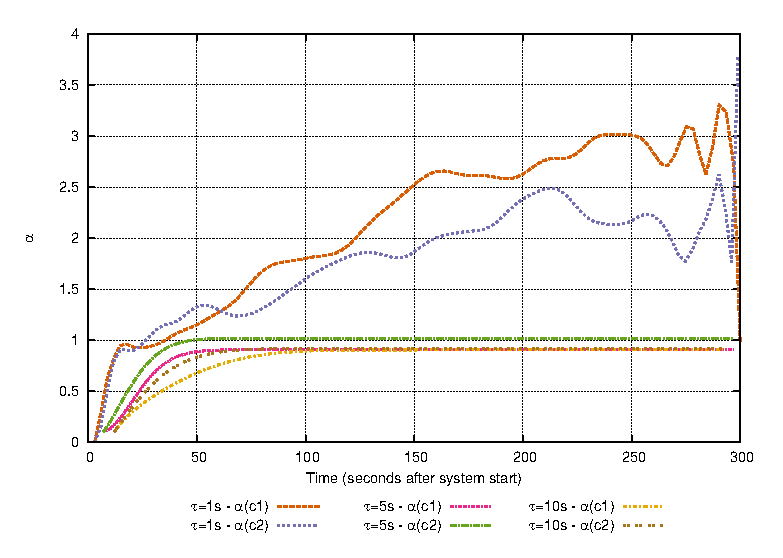
\includegraphics[scale=0.6]{figs/alpha.eps}  
\end{center}
% \vspace{-20pt}
\caption{{\scriptsize Evolving $\alpha(s,\tau,t_c)$ with different $\tau$}}
\label{fig:alpha}
% \vspace{-20pt}
\end{wrapfigure}
%
Every monitoring measurement is performed in a monitoring window $\tau$.
Monitoring measurements are aggregated and calculated in every window and form the basis of reactions necessary to evolve the service to meet their SLA.
Thus, selection of an appropriate monitoring window length $\tau$ is crucial, as we also discussed how schedulability analysis can be used to optimize it.
The authors in \cite{hogben2013defavail} present that for the same setup and deployment of services, measurements using different monitoring windows yield to very different understanding of service properties such as service availability.
Therefore, it is essential to choose the value of $\tau$ such that monitoring measurements do not lead to \emph{unrealistic} understanding and inappropriate reactions.

If $\tau < t_i$, Theorem \ref{thm:alpha} does not hold because every task \jtt{allocate} in $M_{\jtt{A}}$ misses its deadline.
Thus, it is essential that $\tau \geq t_i$.
Analogously, choosing monitoring window as $\tau \gg 2 \times t_i$ also has a counter-productive effect on the service deployments.
% 
% Assumption \ref{def:single:resource:type} says all the resources are of the same type and as such $t_i$ is the same for all resources.
In a real setting, different services may use different types of resources.
In such a setting, the monitoring window should be chosen as the largest $t_i$ of any resource type that is available in the platform: $\tau \geq \mathsf{max}(t_i) \; \forall r \in P$.

% section implementation (end)


% -*- root: paper-esocc.tex -*-

\section{Future work}
\label{ch04:sec:conclusion}


%In this paper, we introduced a distributed monitoring model in order to evolve a service towards its SLA. 
%We formalized characteristics of a distributed service: service availability $\alpha(s,\tau,t_c)$ and service budget compliance $\beta(s,\tau)$.
%We designed task and timed automata for each characteristic to react to the changes of the service in the environment to re-establish its SLA.
%% We presented theorems how SLA for service availability and budget compliance can be met.
%We composed the two characteristics as service sustainability.
%% We showed how the schedulability analsysis of service sustainability builds a model.
%The monitoring model can be used to analyze, model check, and optimize the input parameters to the system (such as $\tau$ and $t_G$), leveraging well-established model checking and schedulability analysis techniques.
%We evaluated the monitoring model on the SDL Fredhopper cloud services.
%We discussed how the results of the evaluation confirm the theorems presented in Section~\ref{ch04:sec:timed:fsm} from a practical standpoint.

% Using the formal model of the service characteristics, we design a monitoring model using actors. 
% Each monitor in the system is responsible for one service.
% Monitors use asynchronous communication through Real-Time ABS to interact with the platform API.
% The monitors observe the system and react to the changes or expectations of the properties. 
% They make changes to the system (\jtt{allocate} or \jtt{deallocate}) through Platform API to ensure the system satisfies its SLA.
% We presented an evaluation of the implementation of the  monitoring platform.
% We showed how choosing certain parameters in the system influences the evolution of the services at runtime.

% There is a wealth of future work for this research.
We continue to generalize the notion of the distributed service characteristics and investigate how the composition of an arbitrary number of such properties can be formalized and reasoned about.
In the context of the ENVISAGE project, industry partners define their service characteristics in this framework and monitor the service evolution.
Moreover, the work will be extended to generate parts of the monitoring platform based on an input of different SLA formalizations such as SLA$\star$~\cite{kearney2010sla}.
Currently, we are integrating our automated monitoring infrastructure
into the in-production SDL Fredhopper cloud services (cf. Section~\ref{ch04:sec:fredhopper_example}).


% \bibliographystyle{abbrv}
% \bibliography{refs}

% \end{document}